\chapter{Desarrollo del proyecto}

Este capítulo presenta el desarrollo técnico realizado para cada una de las tres líneas de trabajo del proyecto, en continuidad con el diseño metodológico del Capítulo~6: clasificación con aprendizaje autosupervisado y adaptación de dominio, segmentación de lesiones cutáneas, y transformación y estimación del tono de piel. Para cada línea se presentan las actividades realizadas, los datos y las entradas, las herramientas, los criterios, el modelamiento matemático y los algoritmos y procedimientos aplicados, incluida la descripción técnica del protocolo de evaluación. Los valores numéricos obtenidos y su interpretación se presentan en el Capítulo~8, que no repite aquí el procedimiento ya descrito.

La Figura~\ref{fig:arquitectura-modular} resume cómo se relacionan entre sí las tres líneas: el clasificador SSL es el núcleo del proyecto, mientras que la segmentación opera como módulo complementario e independiente, con una posible integración (compuerta I) que requiere ablación propia y no se presenta como validada.

\begin{figure}[htbp]
\caption{Arquitectura del clasificador autosupervisado y módulos complementarios de segmentación y adaptación de dominio.}
\label{fig:arquitectura-modular}
\centering
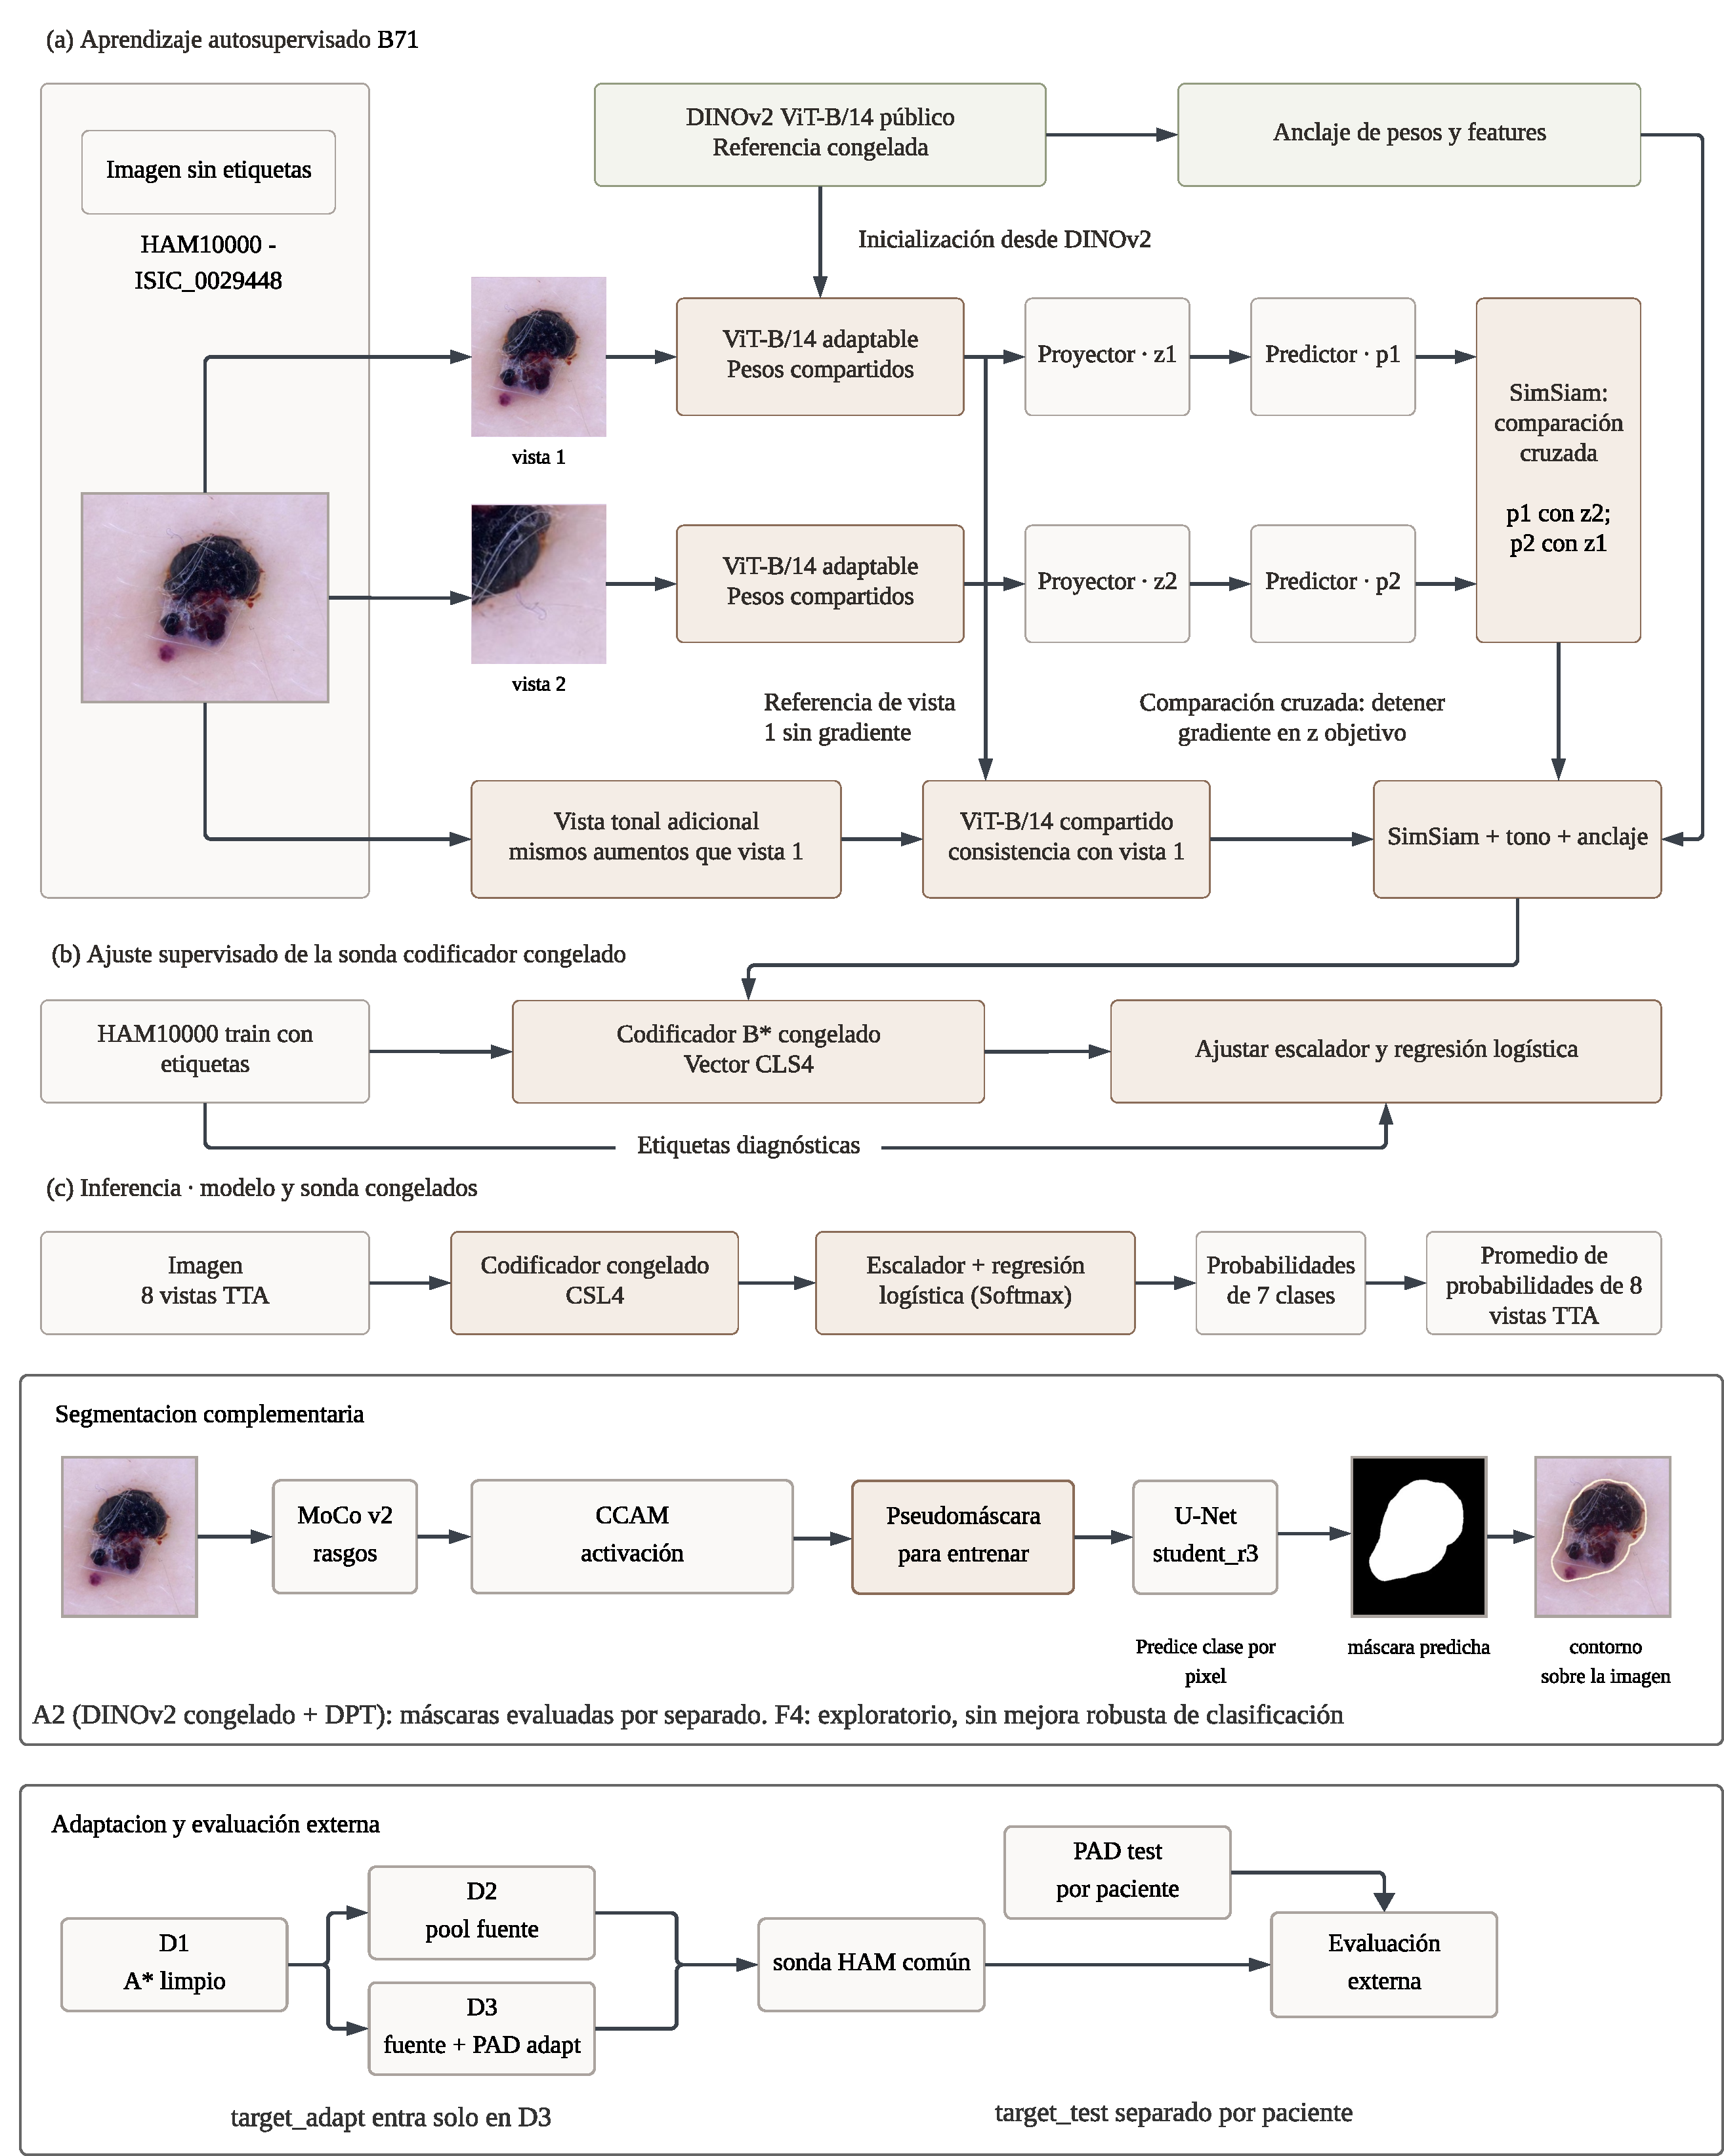
\includegraphics[width=\textwidth,height=0.55\textheight,keepaspectratio]{images/arquitectura-clasificador.pdf}

\par\smallskip
\begingroup\footnotesize\singlespacing\raggedright
\textit{Nota.} Elaboración propia. El diagrama muestra el flujo del clasificador SSL, la segmentación como módulo complementario y las ramas de adaptación de dominio y evaluación externa. El diseño se apoya en DINOv2, SimSiam, MoCo v2 y CCAM \parencite{oquab2024dinov2,chen2021simsiam,chen2020mocov2,xie2022ccam}.
\par\endgroup
\end{figure}

\section{Clasificación con aprendizaje autosupervisado y adaptación de dominio}
\label{sec:desarrollo-clasificador}
Esta línea de trabajo es el núcleo del proyecto: un clasificador de lesiones cutáneas construido sobre un codificador preentrenado de forma autosupervisada y adaptado por dominio hacia el contexto clínico de interés, sin depender de grandes volúmenes de datos etiquetados.

\subsubsection{Actividades y fases}

El desarrollo de esta línea siguió cuatro actividades encadenadas, correspondientes a las fases 1--3 descritas en la sección~\ref{sec:fases-investigacion} y trazadas en la Tabla~\ref{tab:trazabilidad-fases}: (i) selección y caracterización de los conjuntos HAM10000 y PAD-UFES-20; (ii) preentrenamiento autosupervisado del codificador sobre imágenes sin etiqueta, con adaptación de dominio hacia PAD-UFES-20; (iii) ajuste de un clasificador lineal (regresión logística) sobre representaciones congeladas, usando etiquetas de HAM10000; y (iv) evaluación comparativa frente al codificador público, con selección de variantes restringida al conjunto interno y evaluación externa reservada.

\subsubsection{Herramientas y arquitectura}

El codificador base es DINOv2 ViT-B/14, un transformador visual preentrenado públicamente que se adapta mediante SimSiam, el único algoritmo autosupervisado propio de esta línea. ViT-B/14 aporta la arquitectura; SimSiam aporta el procedimiento de adaptación. Se estudiaron dos variantes de adaptación: A* (sin término de consistencia de tono) y B* (con dicho término, descrito en la sección~\ref{sec:modelamiento-clasificador}). Sobre el codificador adaptado, un clasificador lineal (regresión logística) se ajusta con las representaciones y las etiquetas de HAM10000.

Entorno de cómputo del preentrenamiento: cluster UNABIA vía SLURM, 1 nodo con 4 GPU, 32 CPU y 128\,GB de RAM, presupuesto de 40--80 GPU-hora según la variante del \textit{backbone}; Python 3.11, PyTorch 2.4.1, CUDA 12.1, precisión \texttt{bf16}, tamaño de lote efectivo 128, semilla 42.

\subsubsection{Datos y particiones}

HAM10000 es la fuente de entrenamiento y evaluación del clasificador, particionada por \texttt{lesion\_id} para que ninguna lesión aparezca en más de un subconjunto a la vez. PAD-UFES-20 es el dominio objetivo de adaptación: la partición \texttt{target\_adapt} (1.141 imágenes, sin etiquetas) se incorpora al preentrenamiento autosupervisado para continuar adaptando el codificador al dominio clínico; la partición \texttt{target\_test} se reserva íntegramente para evaluación externa y queda excluida de todo entrenamiento, selección de modelos o hiperparámetros, calibración y ajuste de umbrales.

La Figura~\ref{fig:flujo-adaptacion-dominio} presenta el contraste entre D2 y D3. Ambos parten de la misma inicialización y continúan el aprendizaje autosupervisado durante 2.000 pasos; D2 usa el pool fuente y D3 incorpora además 1.141 imágenes clínicas sin etiquetas de \texttt{target\_adapt}, aproximadamente el 2,7\,\% de su pool. Después se congela cada encoder y se ajustan, por condición, el escalador y la regresión logística con las mismas particiones etiquetadas de HAM10000. La comparación final utiliza únicamente \texttt{target\_test}, separado por paciente, sin realimentar el entrenamiento ni la selección. Los resultados de este piloto se presentan en el Capítulo~\ref{chap:resultados}.

\begin{figure}[!htbp]
\caption{Adaptación autosupervisada de dominio: control fuente D2 y condición D3.}
\label{fig:flujo-adaptacion-dominio}
\centering
\includesvg[width=\textwidth]{images/organizadas/20_adaptacion_dominio}
\par\smallskip
\raggedright\fontsize{11}{13}\selectfont\singlespacing
\par\smallskip{\fontsize{11}{13}\selectfont\singlespacing\raggedright
\noindent\textit{Nota.} Elaboración propia a partir del protocolo del proyecto. DINOv2 y SimSiam se apoyan en \textcite{oquab2024dinov2,chen2021simsiam}; PAD-UFES-20 se describe en \textcite{pacheco2020padufes}. La pérdida dibujada resume el objetivo SimSiam; los términos activos adicionales se especifican en el modelamiento matemático. D3 conserva datos fuente además de los clínicos. La evaluación externa comprende 567 imágenes de 363 pacientes y un mapeo parcial BCC/MEL/NV; no constituye validación clínica en Santander.\par}
\par
\end{figure}

\subsubsection{Modelamiento matemático}
\label{sec:modelamiento-clasificador}

Para una imagen $x_i$ y dos vistas aumentadas $v_{i1}$ y $v_{i2}$, el codificador $f_\theta$, el proyector $g_\phi$ y el predictor $q_\psi$ producen
\begin{equation}
 h_{ij}=f_\theta(v_{ij}),\qquad j\in\{1,2\}.
\end{equation}
El proyector transforma la representación del codificador:
\begin{equation}
 z_{ij}=g_\phi(h_{ij}).
\end{equation}
El predictor procesa la salida del proyector:
\begin{equation}
 p_{ij}=q_\psi(z_{ij}).
\end{equation}
La pérdida SimSiam detiene el gradiente en los objetivos $z$ y usa similitud coseno negativa simétrica:
\begin{equation}
 \mathcal L_{\mathrm{SSL}}=-\frac{1}{2N}\sum_{i=1}^{N}\left[
 \frac{p_{i1}^{\mathsf T}\operatorname{sg}(z_{i2})}{\|p_{i1}\|_2\|\operatorname{sg}(z_{i2})\|_2}
 +\frac{p_{i2}^{\mathsf T}\operatorname{sg}(z_{i1})}{\|p_{i2}\|_2\|\operatorname{sg}(z_{i1})\|_2}\right],
\end{equation}
donde $N$ es el tamaño del lote y $\operatorname{sg}$ detiene el gradiente de esa rama.

La variante B* agrega un término de consistencia de tono: una tercera vista $v_{it}$ reutiliza el recorte de la primera vista sobre una copia con tono modificado, y con $h_{it}=f_\theta(v_{it})$,
\begin{equation}
 \mathcal L_{\mathrm{tono}}=\frac{1}{N}\sum_{i=1}^{N}\left[
 1-\frac{h_{it}^{\mathsf T}\operatorname{sg}(h_{i1})}{\|h_{it}\|_2\|\operatorname{sg}(h_{i1})\|_2}\right].
\end{equation}
El entrenamiento ancla los pesos entrenables $\Theta_{\mathrm{ent}}$ hacia su estado inicial $\theta^0$ (L2SP) y las características hacia el codificador público congelado $f_{\theta^0}$:

\noindent Anclaje de parámetros (L2SP): penaliza la distancia cuadrática entre los pesos entrenables y sus valores iniciales.
\begin{equation}
 \mathcal L_{\mathrm{L2SP}}=\sum_{a\in\Theta_{\mathrm{ent}}}(\theta_a-\theta_a^0)^2.
\end{equation}
\noindent Anclaje de representaciones: compara las características aprendidas con las del codificador público congelado sobre la misma vista.
\begin{equation}
 \mathcal L_{\mathrm{dist}}=\frac{1}{N}\sum_{i=1}^{N}\left[
 1-\frac{h_{i1}^{\mathsf T}f_{\theta^0}(v_{i1})}{\|h_{i1}\|_2\|f_{\theta^0}(v_{i1})\|_2}\right].
\end{equation}
\noindent Pérdida total: combina la pérdida base y los términos complementarios con los pesos de la configuración.
\begin{equation}
 \mathcal L_{\mathrm{total}}=\mathcal L_{\mathrm{base}}+\lambda_t\mathcal L_{\mathrm{tono}}+
 \lambda_a\mathcal L_{\mathrm{L2SP}}+\lambda_d\mathcal L_{\mathrm{dist}}.
\end{equation}

Solo se calculan los términos con peso activo en la configuración de la corrida; la variante A* fija $\lambda_t=0$. Según la evaluación consolidada del proyecto, el término de tono (B* frente a A*) no mostró una diferencia demostrable en ningún conjunto evaluado: el aporte medible proviene de la adaptación SSL anclada en sí misma, no del término de tono. El resultado completo se presenta en el Capítulo~\ref{chap:resultados}.

Sobre las representaciones estandarizadas ($u_{ij}=(h_{ij}-\mu_j)/\sigma_j$, con escala unitaria para dimensiones de varianza cero), el clasificador lineal produce
\begin{equation}
 P(y_i=k\mid x_i)=\frac{\exp(w_k^{\mathsf T}u_i+b_k)}{\sum_{c=1}^{7}\exp(w_c^{\mathsf T}u_i+b_c)},
\end{equation}
La predicción corresponde a la clase con mayor probabilidad:
\begin{equation}
 \widehat y_i=\operatorname*{arg\,max}_{k}P(y_i=k\mid x_i).
\end{equation}

\subsubsection{Algoritmo de preentrenamiento}

El Algoritmo~\ref{alg:simsiam-anclado} resume el flujo del clasificador: adaptación autosupervisada, extracción congelada y ajuste de la sonda supervisada.

\begin{algorithm}[htbp]
\fontsize{11}{13}\selectfont\singlespacing
\caption{Flujo del clasificador SSL: adaptación y clasificación}
\label{alg:simsiam-anclado}
\begin{algorithmic}[1]
\State \textbf{Input:} Conjunto de imágenes sin etiqueta $\{x_i\}_{i=1}^N$ (HAM10000 + PAD-UFES-20 \texttt{target\_adapt}); codificador público preentrenado $f_{\theta^0}$; pesos $\lambda_t,\lambda_a,\lambda_d$; número de pasos $T$
\State \textbf{Initialize:} $\theta\leftarrow\theta^0$ \Comment{copia entrenable del codificador público}
\For{$t=1$ \textbf{to} $T$}
  \State Muestrear lote de imágenes; generar vistas aumentadas $v_{i1},v_{i2}$ (y $v_{it}$ si la variante usa término de tono) \Comment{Aumentación}
  \State Calcular $h_{ij}=f_\theta(v_{ij})$, $z_{ij}=g_\phi(h_{ij})$, $p_{ij}=q_\psi(z_{ij})$ \Comment{Paso hacia adelante}
  \State Calcular $\mathcal L_{\mathrm{SSL}}$ con parada de gradiente en $z$ \Comment{Pérdida SimSiam}
  \If{variante B*}
    \State Calcular $\mathcal L_{\mathrm{tono}}$ con $h_{it}$ \Comment{Consistencia de tono}
  \EndIf
  \State Calcular $\mathcal L_{\mathrm{L2SP}}$ y $\mathcal L_{\mathrm{dist}}$ contra $\theta^0$ y $f_{\theta^0}$ \Comment{Anclaje}
  \State $\mathcal L_{\mathrm{total}}\leftarrow \mathcal L_{\mathrm{SSL}}+\lambda_t\mathcal L_{\mathrm{tono}}+\lambda_a\mathcal L_{\mathrm{L2SP}}+\lambda_d\mathcal L_{\mathrm{dist}}$
  \State Actualizar $\theta,\phi,\psi$ por descenso de gradiente sobre $\mathcal L_{\mathrm{total}}$
\EndFor
\State Congelar $f_\theta$ y extraer representaciones de HAM10000
\State Ajustar el escalador y la regresión logística con la partición de entrenamiento etiquetada
\State Aplicar el preprocesamiento fijado y obtener probabilidades de las siete clases
\State Evaluar en las particiones reservadas; no ajustar con \texttt{target\_test}
\State \Return codificador adaptado, escalador y clasificador
\end{algorithmic}
\end{algorithm}

Sobre $f_\theta$ ya adaptado, un clasificador lineal se ajusta por separado con etiquetas de HAM10000 (regresión logística, ecuación anterior); este paso no forma parte del algoritmo autosupervisado.

\subsubsection{Métricas de evaluación}\label{sec:metricas-clasificacion}

Para $K=7$ clases, la matriz de confusión $C\in\mathbb{N}^{K\times K}$ define los conteos de cada clase $k$: $\mathrm{TP}_k=C_{kk}$, $\mathrm{FP}_k=\sum_{l\neq k}C_{lk}$ y $\mathrm{FN}_k=\sum_{l\neq k}C_{kl}$. Las definiciones generales de exactitud, precisión, exhaustividad y F1 se presentan en la Sección~\ref{sec:metricas-evaluacion}; aquí se especifica su aplicación multiclase y las métricas adicionales del proyecto.

\begin{itemize}[label={\raisebox{0.15ex}{\rule{0.45ex}{0.45ex}}},leftmargin=1.5em,labelsep=0.6em,itemsep=0.4\baselineskip,topsep=0.3\baselineskip]
\item Precisión por clase: proporción de predicciones de la clase $k$ que corresponden a esa clase.
\begin{equation}
 \mathrm{Prec}_k=\frac{\mathrm{TP}_k}{\mathrm{TP}_k+\mathrm{FP}_k}.
\end{equation}

\item Exhaustividad por clase: proporción de casos de la clase $k$ que fueron identificados correctamente.
\begin{equation}
 \mathrm{Rec}_k=\frac{\mathrm{TP}_k}{\mathrm{TP}_k+\mathrm{FN}_k}.
\end{equation}

\item F1 por clase: media armónica de la precisión y la exhaustividad de la clase $k$.
\begin{equation}
 F1_k=\frac{2\,\mathrm{Prec}_k\,\mathrm{Rec}_k}{\mathrm{Prec}_k+\mathrm{Rec}_k}.
\end{equation}

\item F1 macro: promedio no ponderado de F1 entre las clases. Es la métrica primaria del proyecto, pues asigna el mismo peso a cada clase.
\begin{equation}
 F1_{\mathrm{macro}}=\frac{1}{K}\sum_{k=1}^{K}F1_k.
\end{equation}

\item Exactitud balanceada: promedio de la sensibilidad de las clases.
\begin{equation}
 \text{Ex. balanceada}=\frac{1}{K}\sum_{k=1}^{K}\mathrm{Rec}_k.
\end{equation}

\item AUC-ROC por clase: en el enfoque uno-contra-el-resto (OvR), compara las puntuaciones $s_i$ de los $n_k^+$ casos positivos y los $n_k^-$ negativos de la clase $k$, contando los empates con peso de un medio.
\begin{equation}
 \mathrm{AUC}_k=\frac{1}{n_k^{+}n_k^{-}}\sum_{i\in k^{+}}\sum_{j\in k^{-}}\left[\mathbb{1}(s_i>s_j)+\tfrac{1}{2}\mathbb{1}(s_i=s_j)\right].
\end{equation}

\item AUC-ROC macro OvR: promedio no ponderado del AUC de las clases.
\begin{equation}
 \mathrm{AUC}_{\mathrm{OvR}}=\frac{1}{K}\sum_{k=1}^{K}\mathrm{AUC}_k.
\end{equation}

\item Error de calibración esperado (ECE): diferencia entre exactitud y confianza en $M$ contenedores $B_m$, ponderada por su número de observaciones.
\begin{equation}
 \mathrm{ECE}=\sum_{m=1}^{M}\frac{|B_m|}{n}\left|\mathrm{acc}(B_m)-\mathrm{conf}(B_m)\right|.
\end{equation}

\item Coeficiente de correlación de Matthews (MCC): medida multiclase calculada con $s$ observaciones, $c$ predicciones correctas, $p_k$ predicciones de la clase $k$ y $t_k$ casos reales de esa clase.
\begin{equation}
 \mathrm{MCC}=\frac{c\cdot s-\sum_{k=1}^{K}p_k t_k}{\sqrt{\left(s^2-\sum_{k=1}^{K}p_k^2\right)\left(s^2-\sum_{k=1}^{K}t_k^2\right)}}.
\end{equation}
\end{itemize}

\subsubsection{Protocolo aplicado antes de los experimentos}\label{sec:protocolo-estadistico}

Antes de ejecutar cualquier comparación confirmatoria se congelan los manifiestos (identificadores, hashes y exclusiones de cada partición), se fija la separación por \texttt{lesion\_id} y se registran de antemano el conjunto de datos, la arquitectura, el preprocesamiento, las particiones, las semillas y la regla de decisión. La Figura~\ref{fig:protocolo-evaluacion} resume la secuencia de adaptación, ajuste supervisado e inferencia, incluida la separación entre la selección de variantes en el conjunto interno y la evaluación externa reservada en PAD-UFES-20 \texttt{target\_test}.

\begin{figure}[!htbp]
\caption{Protocolo de clasificación, adaptación de dominio y evaluación externa.}
\label{fig:protocolo-evaluacion}
\centering
\includesvg[width=\textwidth]{images/organizadas/21_protocolo_vertical}

\par\smallskip
\begingroup\footnotesize\singlespacing\raggedright
\par\smallskip{\fontsize{11}{13}\selectfont\singlespacing\raggedright
\noindent\textit{Nota.} Elaboración propia. El esquema se centra en el protocolo de clasificación y adaptación: D2 continúa SimSiam con el pool fuente; D3 añade \texttt{target\_adapt} a ese pool. HAM10000 aporta el ajuste supervisado y la validación interna. Cada condición ajusta su propio escalador y regresión logística; la referencia utiliza el encoder público sin adaptación. \texttt{target\_test} solo interviene en la inferencia y evaluación, con separación por paciente y sin reajuste. El esquema se apoya en DINOv2 y SimSiam \parencite{oquab2024dinov2,chen2021simsiam}. Los procedimientos de segmentación y tono se presentan en sus secciones específicas.\par}
\par\endgroup
\end{figure}

 Las comparaciones pareadas usan remuestreo bootstrap por lesión ($B=1\,000$ remuestras) con intervalo de confianza al 95\,\% por el método percentil, y corrección de Holm para contrastes múltiples: ordenados los valores $p_{(1)}\leq\cdots\leq p_{(m)}$, se rechaza la hipótesis asociada a $p_{(i)}$ si $p_{(i)}\leq \alpha/(m-i+1)$, deteniendo el procedimiento en el primer índice donde la condición falla.

Este protocolo responde directamente a cuatro riesgos de integridad de la evidencia identificados para esta línea:
\begin{itemize}
 \item \textbf{Solapamiento de imágenes de una lesión entre particiones}, que produciría fuga de información y métricas optimistas: se controla separando por \texttt{lesion\_id} y congelando listas y hashes antes de entrenar.
 \item \textbf{Bootstrap por imagen en HAM10000}, que produciría intervalos demasiado estrechos por correlación intralesión: se reporta esta limitación y se complementa con un análisis de sensibilidad agrupado por lesión antes de afirmaciones confirmatorias.
 \item \textbf{Conjuntos de datos y modalidades diferentes} (HAM10000 dermatoscópico frente a PAD-UFES-20 clínico), que podrían simular una transferencia aparente o un deterioro fuera de dominio: se describe la modalidad, la fuente y la población de cada conjunto, y PAD-UFES-20 se reporta por separado.
 \item \textbf{Línea base supervisada con partición distinta}, que haría la comparación no pareada y no atribuible solo al régimen de aprendizaje: se iguala el conjunto de datos, la arquitectura, la partición, el presupuesto de cómputo y las métricas antes de concluir.
\end{itemize}



\section{Segmentación de lesiones cutáneas}
\label{sec:desarrollo-segmentacion}
Esta línea de trabajo es un módulo complementario al clasificador: genera, sin usar máscaras expertas ni etiquetas de diagnóstico en ningún punto del proceso, una segmentación aproximada de la lesión que puede alimentar al módulo de incertidumbre y a la caracterización de tono descrita en la Sección~\ref{sec:desarrollo-tono}. No sustituye una validación clínica de la segmentación.

\subsubsection{Actividades y fases}

El \textit{pipeline} se organiza en dos etapas secuenciales dentro de la Fase 2 de la Tabla~\ref{tab:trazabilidad-fases}: una generación inicial de la pseudo-máscara y un refinamiento iterativo que repite el entrenamiento del U-Net estudiante sobre versiones sucesivamente mejoradas de esa pseudo-máscara.

\begin{enumerate}
    \item \textbf{Generación inicial.}
    \begin{enumerate}
        \item \textbf{\texttt{contrastive}}: preentrenamiento contrastivo del \textit{backbone} con MoCo v2 (algoritmo de MoCo v2 más abajo), sin etiquetas.
        \item \textbf{\texttt{ccam}}: generación del mapa de activación de clase agnóstica con CCAM (algoritmo de CCAM más abajo) a partir de las representaciones de \texttt{contrastive}.
        \item \textbf{\texttt{pseudo\_r0}}: umbralización del mapa CCAM para producir la primera pseudo-máscara.
        \item \textbf{\texttt{student\_r1}}: entrenamiento de un U-Net estudiante sobre \texttt{pseudo\_r0}.
    \end{enumerate}
    \item \textbf{Refinamiento iterativo.} Cada ronda repite el mismo patrón hasta llegar a \texttt{student\_r3}: refinar la pseudo-máscara con las predicciones del estudiante de la ronda anterior y entrenar sobre ella una nueva ronda de U-Net estudiante.
    \begin{enumerate}
        \item \textbf{\texttt{pseudo\_r1}}: refinamiento de la pseudo-máscara con las predicciones de \texttt{student\_r1}.
        \item \textbf{\texttt{student\_r2}}: segunda ronda de entrenamiento del U-Net sobre \texttt{pseudo\_r1}.
        \item \textbf{\texttt{pseudo\_r2}}: segundo refinamiento de la pseudo-máscara.
        \item \textbf{\texttt{student\_r3}}: tercera y última ronda de entrenamiento del U-Net sobre \texttt{pseudo\_r2}; es el candidato final de este módulo.
    \end{enumerate}
\end{enumerate}

Las tres rondas de estudiante (\texttt{student\_r1}--\texttt{student\_r3}) comparten el mismo protocolo de entrenamiento: 20 épocas, 32 imágenes por GPU en 2 GPU, optimizador Adam con tasa de aprendizaje $10^{-4}$, una época de calentamiento, programación coseno, precisión \texttt{bf16} y semilla 42. La pérdida combina entropía cruzada binaria y Dice suave, calculada solo sobre los píxeles que el módulo de incertidumbre marca como confiables.

\texttt{student\_r3} se tomó como candidato final por ser la última ronda ejecutada, no por una comparación de métricas entre \texttt{student\_r1}, \texttt{student\_r2} y \texttt{student\_r3}. La configuración registrada especifica tres rondas de re-etiquetado, 20 épocas por ronda de estudiante y 30 épocas contrastivas. Los artefactos no incluyen una comparación experimental entre distintos números de rondas ni documentan por qué se fijaron exactamente tres; por tanto, no se presenta esa cantidad como óptima. El equipo informó que el tiempo disponible limitó la exploración de variantes adicionales, lo cual se reporta como limitación experimental y no como justificación documentada del número de rondas. Dentro de cada ronda, el punto de verificación se seleccionó según la pérdida de pseudo-validación.

\subsubsection{Herramientas y arquitectura}

El \textit{backbone} es un ResNet-50 preentrenado de forma contrastiva con MoCo v2 \parencite{chen2020mocov2}, independiente del SimSiam que adapta el \textit{backbone} del clasificador (Sección~\ref{sec:desarrollo-clasificador}). Sobre ese \textit{backbone}, CCAM (\emph{Contrastive learning of Class-agnostic Activation Maps}, \parencite{xie2022ccam}) produce un mapa de activación sin etiquetas de segmentación, que se umbraliza para entrenar al U-Net estudiante. \textit{Framework} y \textit{hardware}: ver configuración experimental en el Capítulo~\ref{chap:resultados}; a diferencia del preentrenamiento del clasificador (cluster UNABIA vía SLURM, 4 GPU), este módulo se ejecuta en un pod Jupyter con 2 GPU RTX PRO 4000 Blackwell de 24GB, CUDA 13.0 y \texttt{torch 2.11.0+cu128} --una versión de PyTorch distinta a la del clasificador porque son dos entornos de cómputo independientes, no por inconsistencia.

\paragraph{Alternativa S4-A2.} Como variante posterior se evaluó un \textit{decoder} tipo DPT con un \textit{encoder} público DINOv2 ViT-B/14 congelado. El \textit{decoder} combina las salidas de los bloques 3, 6, 9 y 12 y se entrena con las pseudo-máscaras iniciales \texttt{pseudo\_r0} generadas por CCAM, sin máscaras expertas. Su criterio, registrado antes de la evaluación, fue alcanzar en ISIC2018 un Dice no inferior a \texttt{student\_r3} por más de 0,01; se evalúa además en HAM10000. S4-A2 es una alternativa distinta del refinamiento iterativo \texttt{student\_r1}--\texttt{student\_r3}, no una cuarta ronda.

\subsubsection{Datos empleados}

\begin{sloppypar}
El \textit{pool} desduplicado de imágenes sin etiquetas contiene 58.457 imágenes: 10.015 de HAM10000, 15.316 de ISIC2019 que no duplican HAM10000 y 33.126 de ISIC2020. Esta cifra corresponde al módulo de segmentación y no al \textit{pool} de preentrenamiento del clasificador. Para la caché compartida por \texttt{student\_r3} y S4-A2, el registro de ejecución especifica 57.288 imágenes de entrenamiento y 1.169 de pseudo-validación; de ellas, 52.453 y 1.082, respectivamente, cuentan con píxeles confiables. En \texttt{pseudo\_r2}, 2.508 imágenes (4,29\,\%) quedaron excluidas por los criterios de región y área de la máscara. Ninguna etapa de entrenamiento utiliza las máscaras expertas de ISIC2018 ni etiquetas de diagnóstico. La evaluación final compara las predicciones con máscaras de referencia de ISIC2018 (2.594 imágenes) y HAM10000 (10.015). Como parte de ISIC2018 coincide por identificador con imágenes incluidas sin etiquetas en el \textit{pool}, esta evaluación es parcialmente transductiva y no debe describirse como completamente independiente.
\end{sloppypar}

\subsubsection{Criterios de evaluación}

La selección de cada punto de verificación de \texttt{student\_r1}--\texttt{student\_r3} se basa en la pérdida de pseudo-validación, no en las máscaras expertas. La evaluación posterior contra las máscaras de referencia reporta Dice, IoU, sensibilidad, especificidad y distancia de Hausdorff al percentil 95 (HD95). Para S4-A2 se fijó antes de la evaluación el umbral de adopción Dice $\geq$ Dice(\texttt{student\_r3}) $-0{,}01$ en ISIC2018; cumplirlo permite considerarlo candidato de segmentación, pero no demuestra una mejora del clasificador. El coeficiente Dice entre la máscara predicha $A$ y la máscara de referencia $B$ se define como:
\begin{equation}
 \mathrm{Dice}(A,B)=\frac{2|A\cap B|}{|A|+|B|}=\frac{2\,\mathrm{TP}}{2\,\mathrm{TP}+\mathrm{FP}+\mathrm{FN}},
 \label{eq:dice-s6}
\end{equation}
donde $\mathrm{TP}$, $\mathrm{FP}$ y $\mathrm{FN}$ se calculan a nivel de píxel entre ambas máscaras. Los valores de Dice obtenidos se presentan como resultado en el Capítulo~7, no en este apartado.

\subsubsection{Modelamiento matemático}

\paragraph{MoCo v2.} Un codificador de consulta $f_q$ procesa la vista $x^q$ y un codificador de clave $f_k$, actualizado por media móvil exponencial del codificador de consulta ($\theta_k\leftarrow m\,\theta_k+(1-m)\theta_q$, con $m=0{,}99$), procesa la vista $x^k$. Las representaciones $q=f_q(x^q)$ y $k=f_k(x^k)$ se comparan contra una cola de $Q=16\,384$ claves negativas $\{k_j\}_{j=1}^{Q}$ acumuladas de lotes anteriores, con temperatura $\tau=0{,}2$:
\begin{equation}
 \mathcal L_{\mathrm{MoCo}}=-\log\frac{\exp(q\cdot k_+/\tau)}{\exp(q\cdot k_+/\tau)+\sum_{j=1}^{Q}\exp(q\cdot k_j/\tau)}.
 \label{eq:moco-loss-s6}
\end{equation}
Los parámetros de $f_k$ no reciben gradiente directo; solo se actualizan por la media móvil.

\paragraph{CCAM.} Para un mapa de características $Z\in\mathbb{R}^{C\times h\times w}$ del \textit{backbone} y un mapa de activación $P\in(0,1)^{1\times h\times w}=\sigma(\mathrm{BN}(\mathrm{Conv}(Z)))$, los vectores de primer plano y de fondo son promedios ponderados espacialmente:
\begin{equation}
 v_f=\operatorname{norm}\left(\sum_{p} P(p)\,Z(p)\right),\qquad
 v_b=\operatorname{norm}\left(\sum_{p}\bigl(1-P(p)\bigr)\,Z(p)\right).
 \label{eq:ccam-vectores-s6}
\end{equation}
La pérdida combina un término negativo (separar primer plano de fondo dentro de la misma imagen) y uno positivo (acercar primeros planos entre sí y fondos entre sí, ponderado por similitud dentro del lote):
\begin{align}
 \mathcal L_{\mathrm{NEG}}&=-\frac{1}{B}\sum_{i=1}^{B}\log\left(1-v_f^{(i)\top}v_b^{(i)}\right),\\
 \mathcal L_{\mathrm{POS}}&=-\frac{1}{B(B-1)}\sum_{i\neq j} w_{ij}\log\left(v_f^{(i)\top}v_f^{(j)}\right) + \text{(término análogo para } v_b\text{)},
\end{align}
con peso $w_{ij}=\exp(-\alpha\cdot\operatorname{rank}_{ij})$, de modo que solo los pares más parecidos del lote contribuyen de forma apreciable. La pérdida total es $\mathcal L_{\mathrm{CCAM}}=\mathcal L_{\mathrm{POS}}+\mathcal L_{\mathrm{NEG}}$. El mapa $P$ resultante se umbraliza para producir la pseudo-máscara inicial.

\subsubsection{Algoritmos}

\begin{algorithm}[htbp]
\caption{MoCo v2 (preentrenamiento contrastivo del backbone)}
\label{alg:mocov2}
\begin{algorithmic}[1]
\Statex \textbf{Input:} lote de imágenes sin etiquetar; dos aumentaciones por imagen $x^q$, $x^k$
\Statex \textbf{Initialize:} codificador de consulta $f_q$; codificador de clave $f_k\leftarrow f_q$; cola vacía de $Q=16\,384$ claves; $m=0{,}99$; $\tau=0{,}2$
\For{cada lote}
  \State $q\leftarrow f_q(x^q)$,\ $k\leftarrow f_k(x^k)$ \Comment{sin gradiente por $f_k$}
  \State Calcular $\mathcal L_{\mathrm{MoCo}}$ (Ecuación~\ref{eq:moco-loss-s6}) con la cola actual \Comment{paso de pérdida}
  \State Actualizar $f_q$ por descenso de gradiente sobre $\mathcal L_{\mathrm{MoCo}}$ \Comment{solo $f_q$ recibe gradiente}
  \State $\theta_k\leftarrow m\,\theta_k+(1-m)\,\theta_q$ \Comment{actualización por media móvil}
  \State Encolar $k$; descartar la clave más antigua si la cola excede $Q$ \Comment{actualización de la cola}
\EndFor
\State \Return backbone ResNet-50 preentrenado $f_q$
\end{algorithmic}
\end{algorithm}

\begin{algorithm}[htbp]
\caption{CCAM (generación de pseudo-máscaras)}
\label{alg:ccam}
\begin{algorithmic}[1]
\Statex \textbf{Input:} lote de $B$ imágenes; backbone preentrenado (Algoritmo~\ref{alg:mocov2})
\Statex \textbf{Initialize:} capa convolucional + BN + sigmoide sobre el mapa de características $Z$
\For{cada lote}
  \State $P\leftarrow\sigma(\mathrm{BN}(\mathrm{Conv}(Z)))$ \Comment{mapa de activación}
  \State Calcular $v_f$, $v_b$ (Ecuación~\ref{eq:ccam-vectores-s6}) \Comment{vectores primer plano/fondo}
  \State Calcular $\mathcal L_{\mathrm{CCAM}}=\mathcal L_{\mathrm{POS}}+\mathcal L_{\mathrm{NEG}}$ \Comment{paso de pérdida}
  \State Actualizar los pesos de la capa por descenso de gradiente \Comment{paso de optimización}
\EndFor
\State Umbralizar $P$ \Comment{pseudo-máscara inicial (\texttt{pseudo\_r0})}
\State \Return pseudo-máscara inicial para entrenar al U-Net estudiante
\end{algorithmic}
\end{algorithm}


\section{Transformación y estimación del tono de piel}
\label{sec:desarrollo-tono}
Esta línea de trabajo comprende dos procedimientos distintos que comparten el mismo espacio de color (CIELAB) pero cumplen funciones diferentes dentro del proyecto: la \textbf{estimación} del ángulo de tipología individual (ITA) como proxy colorimétrico para caracterizar los conjuntos de datos, y la \textbf{transformación} determinística de tono usada como augmentación durante el preentrenamiento SSL del clasificador (brazo B*, sección~\ref{sec:desarrollo-clasificador}). Ninguno de los dos procedimientos es un modelo entrenado: ambos son operaciones de cómputo directo sobre los canales CIELAB de cada imagen, sin parámetros que se ajusten con datos.

\subsection{Actividades y datos}

Las actividades de esta línea, ejecutadas dentro de las Fases 2 y 3 de la Tabla~\ref{tab:trazabilidad-fases}, fueron: (i) calcular el proxy ITA por imagen sobre los conjuntos HAM10000, ISIC2019 e ISIC2020 para caracterizar su distribución de tono; (ii) aplicar la transformación determinística de tono como augmentación de la tercera vista del brazo B* durante el preentrenamiento SimSiam; y (iii) validar el proxy ITA contra fototipo Fitzpatrick (FST) real en dos conjuntos externos con anotación experta. Los datos usados son los mismos conjuntos de la línea de clasificación (HAM10000, 10.015 imágenes; pool local de ISIC2019, 15.316 imágenes; pool local de ISIC2020, 33.126 imágenes) más dos conjuntos externos exclusivos de validación: Fitzpatrick17k-C (11.098 imágenes con FST asignado por expertos) y la partición de PAD-UFES-20 con fototipo clínico disponible (1.494 de 2.298 imágenes totales).

\subsection{Estimación del ángulo de tipología individual (ITA)}

El ITA se calcula sobre píxeles de piel seleccionados por máscara, usando las medianas de los canales CIELAB $L^*$ y $b^*$ de la región muestreada:
\begin{equation}
 \mathrm{ITA}=\frac{180}{\pi}\arctan\!\left(\frac{\widetilde L^*-50}{\widetilde b^*}\right).
\end{equation}
El cálculo se repite sobre tres regiones de muestreo de piel por imagen --máscara por Otsu, imagen completa y anillo perilesional--, usando pseudo-máscaras automáticas del segmentador (sección~\ref{sec:desarrollo-segmentacion}) cuando están disponibles. El resultado se marca como indeterminado si $\widetilde b^*<5$, y la imagen queda en cuarentena cuando no hay piel suficiente o la máscara es degenerada.

\begin{algorithm}[htbp]
\caption{Estimación del ángulo de tipología individual (ITA)}
\label{alg:estimacion-ita}
\begin{algorithmic}[1]
\Statex \textbf{Input:} Imagen $x$ a resolución canónica, máscara de piel candidata $M_s$ (Otsu, imagen completa o anillo perilesional), pseudo-máscara de lesión del segmentador (si disponible)
\Statex \textbf{Initialize:} región de muestreo $R \gets M_s \setminus \text{lesión}$
\If{$|R|$ insuficiente \textbf{or} máscara degenerada}
  \State \Return indeterminado \Comment{abstención explícita, imagen en cuarentena}
\EndIf
\State Convertir $x$ a CIELAB y restringir a $R$
\State $\widetilde L^* \gets$ mediana de $L^*$ en $R$ \Comment{robusto a artefactos puntuales}
\State $\widetilde b^* \gets$ mediana de $b^*$ en $R$
\If{$\widetilde b^* < 5$}
  \State \Return indeterminado \Comment{denominador numéricamente inestable}
\EndIf
\State $\mathrm{ITA} \gets (180/\pi)\arctan\!\big((\widetilde L^*-50)/\widetilde b^*\big)$
\State \Return $\mathrm{ITA}$ \Comment{proxy colorimétrico, no un fototipo clínico}
\end{algorithmic}
\end{algorithm}

\subsection{Transformación determinística de tono}

La transformación recibe una máscara de lesión $M(p)$ (valor uno en la lesión) y un desplazamiento entero solicitado $s$, acotado a $s_c=\max(-2,\min(2,s))$. Modifica el canal CIELAB $L^*$ únicamente fuera de la lesión:
\begin{equation}
 L^{*\prime}(p)=\begin{cases}
 L^*(p), & M(p)=1,\\
 \operatorname{clip}\big(L^*(p)-8s_c,\,0,\,100\big), & M(p)=0.
 \end{cases}
\end{equation}
Los canales $a^*$ y $b^*$ se conservan sin cambios. Es una operación \textbf{determinística}: no hay parámetros aprendidos ni ajuste con datos, solo un desplazamiento fijo de luminosidad seguido de recorte a rango válido.

\begin{algorithm}[htbp]
\caption{Transformación determinística de tono de piel}
\label{alg:transformacion-tono}
\begin{algorithmic}[1]
\Statex \textbf{Input:} Imagen $x$ en sRGB, máscara de lesión $M$, desplazamiento solicitado $s$
\Statex \textbf{Initialize:} $s_c \gets \max(-2,\min(2,s))$ \Comment{acotar el desplazamiento}
\If{máscara no elegible según el manifiesto}
  \State \Return rechazar \Comment{versión protegida por manifiesto}
\EndIf
\State Convertir $x$ de sRGB a CIELAB $(L^*,a^*,b^*)$
\For{cada píxel $p$}
  \If{$M(p)=1$}
    \State $L^{*\prime}(p) \gets L^*(p)$ \Comment{lesión sin modificar}
  \Else
    \State $L^{*\prime}(p) \gets \operatorname{clip}(L^*(p)-8s_c,\,0,\,100)$ \Comment{incluye fondo y artefactos}
  \EndIf
\EndFor
\State Convertir $(L^{*\prime},a^*,b^*)$ de CIELAB a sRGB
\State Restaurar exactamente los píxeles originales dentro de $M$
\State Acotar el resultado a $[0,1]$
\State \Return imagen transformada en sRGB
\end{algorithmic}
\end{algorithm}

La operación modifica todos los píxeles fuera de la máscara de lesión, incluidos el fondo y los artefactos que permanezcan allí; no utiliza una selección adicional que identifique exclusivamente piel. Por ello, el desplazamiento representa una \textbf{modificación sintética de luminosidad}, no una corrección validada del tono de piel: no cambia el fototipo clínico de la imagen ni garantiza el paso a otro fototipo. Esta transformación alimenta únicamente la tercera vista del brazo B* durante el preentrenamiento (pérdida $\mathcal L_{\mathrm{tono}}$, sección~\ref{sec:desarrollo-clasificador}); no se usa en el pipeline de estimación de ITA de la subsección anterior.

\subsection{Validación externa y limitaciones}

El proxy ITA \textbf{no está validado} como estimador del fototipo Fitzpatrick real. En Fitzpatrick17k-C (11.098 imágenes con FST experto), la exactitud del proxy fue de 28,5\,\% a 30,8\,\%, frente a 32,9\,\% de la línea base por mayoría. En la evaluación exploratoria propia de PAD-UFES-20 se partió de 1.494 registros con fototipo clínico válido. Para la imagen completa, 1.265 casos tuvieron estimación y 229 no; la exactitud fue 21,74\,\% (IC del 95\,\%: 19,18\,\%--24,48\,\%), frente a 59,37\,\% de la línea base calculada sobre los mismos casos. Con el fondo enmascarado mediante Otsu, 1.189 casos tuvieron estimación y 305 no; la exactitud fue 22,88\,\% (IC del 95\,\%: 20,12\,\%--25,88\,\%), frente a 59,80\,\% de la línea base para esos mismos casos. Las cifras de 22,9\,\% y 51,3\,\% corresponden a un estudio de Alipour et al. (2026) con condiciones distintas, no a la validación propia \parencite{alipour2026italimitations}. En ambas evaluaciones del proyecto, el ITA quedó por debajo de la línea base por mayoría; no hay evidencia de que represente el fototipo clínico mejor que predecir la clase más frecuente.

Esta limitación corresponde al riesgo de evidencia \textit{ITA presentado como fototipo}: nombrarlo incorrectamente como FST produciría conclusiones inválidas sobre equidad por fototipo. El control aplicado en este documento y en el repositorio es nombrar siempre el proxy como ITA y no afirmar fototipo Fitzpatrick sin anotación experta y validación --como se hace en esta sección y en la caracterización de conjuntos del Capítulo~8 (Sección~\ref{sec:caracterizacion-tono}).

La comparación entre Otsu, la imagen completa y el anillo perilesional es descriptiva: los registros disponibles no incluyen una máscara de piel experta que permita medir cuál región estima mejor la piel, ni un criterio validado para seleccionar una de ellas. La cobertura, las abstenciones y las diferencias de ITA se reportan como características operacionales, no como validación de calidad ni como asignación de fototipo. Por esta razón, esta comparación no sustenta afirmaciones de equidad por tono de piel.

